\documentclass[12pt,a4paper]{article}

% ── Packages ──────────────────────────────────────────────────────────────────
\usepackage[margin=2.5cm]{geometry}
\usepackage{graphicx}
\usepackage{subcaption}
\usepackage{booktabs}
\usepackage{array}
\usepackage{multirow}
\usepackage{tabularx}
\usepackage{amsmath}
\usepackage{amssymb}
\usepackage{algorithm}
\usepackage{algpseudocode}
\usepackage{hyperref}
\usepackage{xcolor}
\usepackage{caption}
\usepackage{float}
\usepackage{enumitem}
\usepackage{setspace}
\usepackage{fancyhdr}
\usepackage{titlesec}
\usepackage{parskip}
\usepackage{tikz}
\usetikzlibrary{shapes.geometric, arrows.meta, positioning, fit, backgrounds, calc}

% ── Colors ────────────────────────────────────────────────────────────────────
\definecolor{darkblue}{RGB}{0,51,102}
\definecolor{lightblue}{RGB}{210,228,245}
\definecolor{nodegreen}{RGB}{200,230,200}
\definecolor{nodeap}{RGB}{255,225,180}
\definecolor{nodehead}{RGB}{220,210,240}

% ── Hyperref ──────────────────────────────────────────────────────────────────
\hypersetup{
    colorlinks=true,
    linkcolor=blue!70!black,
    citecolor=green!50!black,
    urlcolor=cyan!70!black,
    pdftitle={TCP NewReno+ Modified: Project Report},
    pdfauthor={Nayeem Uz Zaman}
}

% ── Header/Footer ─────────────────────────────────────────────────────────────
\pagestyle{fancy}
\fancyhf{}
\rhead{\textit{TCP NewReno$^+$ Modified — Project Report}}
\lhead{\textit{Nayeem Uz Zaman | 2105090}}
\cfoot{\thepage}
\renewcommand{\headrulewidth}{0.4pt}

% ── Section formatting ────────────────────────────────────────────────────────
\titleformat{\section}{\large\bfseries\color{darkblue}}{\thesection.}{0.5em}{}[\titlerule]
\titleformat{\subsection}{\normalsize\bfseries}{\thesubsection}{0.5em}{}
\titleformat{\subsubsection}{\normalsize\itshape\bfseries}{\thesubsubsection}{0.5em}{}

% ── Graphics path ─────────────────────────────────────────────────────────────
\graphicspath{{plots/}}

% ── Algorithm style ───────────────────────────────────────────────────────────
\algrenewcommand\algorithmiccomment[1]{\hfill\textcolor{gray}{\small\textit{// #1}}}

% ══════════════════════════════════════════════════════════════════════════════
\begin{document}
% ══════════════════════════════════════════════════════════════════════════════

% ── Title Page ────────────────────────────────────────────────────────────────
\begin{titlepage}
    \centering
    \vspace*{1.2cm}
    {\LARGE\bfseries Project Report\par}
    \vspace{0.4cm}
    \rule{0.85\linewidth}{1.2pt}
    \vspace{0.4cm}
    {\Large\bfseries Implementation and Enhancement of\\[0.4em]
    TCP NewReno\textsuperscript{+} in NS-3\par}
    \vspace{0.3cm}
    \rule{0.85\linewidth}{0.5pt}
    \vspace{1.2cm}

    {\large
    \begin{tabular}{rl}
        \textbf{Student Name:} & Nayeem Uz Zaman \\[4pt]
        \textbf{Student ID:}   & 2105090 \\[4pt]
        \textbf{Department:}   & Computer Science and Engineering \\[4pt]
        \textbf{Platform:}     & ns-3 (version 3.45) \\[4pt]
        \textbf{Date:}         & April 2026 \\
    \end{tabular}
    }

    \vspace{1.5cm}
    \rule{0.85\linewidth}{0.5pt}
    \vspace{0.8cm}

    \begin{minipage}{0.85\textwidth}
    \textbf{Paper Reference:}\\[0.4em]
    Ahmed Khurshid, Md.\ Humayun Kabir, and Rajkumar Das,
    ``\textit{Modified TCP NewReno for Wireless Networks},''
    IEEE International Conference on Networking Systems and Security, 2015.
    \end{minipage}

    \vfill
    {\small Department of Computer Science and Engineering\\
    Bangladesh University of Engineering and Technology}
\end{titlepage}


% ══════════════════════════════════════════════════════════════════════════════
\section{Paper Description}
% ══════════════════════════════════════════════════════════════════════════════

Standard TCP treats every packet loss as a signal of network congestion, shrinking
the congestion window regardless of the true cause. In wired networks this is
largely correct — virtually all losses come from router-buffer overflow.
In wireless networks, however, random bit errors, channel fading, and physical-layer
collisions cause losses that have nothing to do with congestion. When TCP reacts to
these losses by throttling the sender, it wastes available bandwidth without
alleviating any real problem. The paper calls this the \textbf{Loss Ambiguity}
problem.

Khurshid \textit{et al.}\ (2015) propose \textbf{TCP NewReno+}, which adds two
statistical counters to track the history of loss events. Two ratios derived from
these counters — the \emph{Timeout-to-Dupack Ratio} (TDR) and the
\emph{Inter-Timeout Ratio} (ITR) — are used to probabilistically classify each
loss event as either a genuine congestion event (which warrants window reduction)
or a wireless bit-error event (which does not). The algorithm is tested in ns-2 on
a mixed wired–wireless topology and outperforms TCP NewReno and TCP Westwood.

% ══════════════════════════════════════════════════════════════════════════════
\section{Network Topology (Paper Replication)}
\label{sec:paper-topo}
% ══════════════════════════════════════════════════════════════════════════════

The paper uses a \textbf{mixed wired–wireless topology}: three wired senders and
one gateway/access-point node connect to a head node over dedicated 5\,Mbps
point-to-point links. The gateway links to the head node via a configurable
bottleneck. Five wireless nodes associate with the access point over an
IEEE\,802.11b link with a tunable packet error rate. Two UDP CBR background flows
inject congestion.

\begin{itemize}[noitemsep]
  \item \textbf{Single-flow:} 1 TCP connection (S$_1 \to$ R$_1$);
        bottleneck = 7\,Mbps.
  \item \textbf{Multi-flow:} 2 concurrent TCP connections;
        bottleneck = 12\,Mbps.
  \item Simulation time: 250\,s; segment size: 1000\,bytes; TCP buffer: 2\,MB.
\end{itemize}

\begin{figure}[H]
\centering
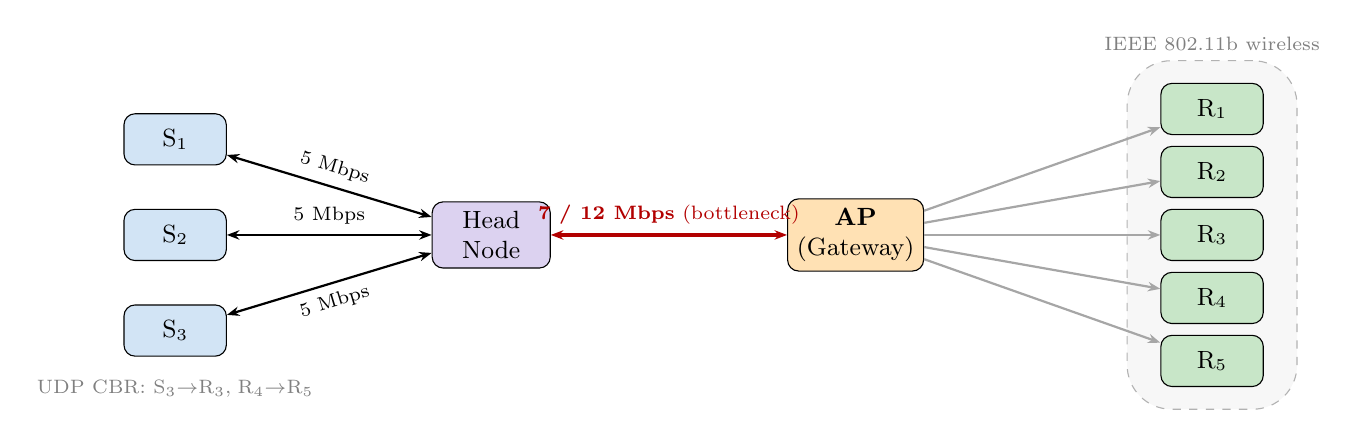
\begin{tikzpicture}[
    node distance = 1.5cm and 2.4cm,
    every node/.style = {font=\small},
    senderbox/.style  = {draw, rounded corners=4pt, fill=lightblue,
                         minimum width=1.3cm, minimum height=0.65cm, align=center},
    headbox/.style    = {draw, rounded corners=4pt, fill=nodehead,
                         minimum width=1.5cm, minimum height=0.65cm, align=center},
    apbox/.style      = {draw, rounded corners=4pt, fill=nodeap,
                         minimum width=1.5cm, minimum height=0.65cm, align=center},
    rcvbox/.style     = {draw, rounded corners=4pt, fill=nodegreen,
                         minimum width=1.3cm, minimum height=0.65cm, align=center},
    arr/.style        = {-{Stealth[length=4.5pt]}, thick},
    darr/.style       = {{Stealth[length=4.5pt]}-{Stealth[length=4.5pt]}, thick},
]

% Senders
\node[senderbox] (S1) {S$_1$};
\node[senderbox, below=0.55cm of S1] (S2) {S$_2$};
\node[senderbox, below=0.55cm of S2] (S3) {S$_3$};

% Head node — centred on S2
\node[headbox, right=2.6cm of S2] (HN) {Head\\Node};

% AP
\node[apbox, right=3.0cm of HN] (AP) {\textbf{AP}\\(Gateway)};

% Wireless receivers
\node[rcvbox, right=3.0cm of AP, yshift= 1.6cm] (R1) {R$_1$};
\node[rcvbox, right=3.0cm of AP, yshift= 0.8cm] (R2) {R$_2$};
\node[rcvbox, right=3.0cm of AP, yshift= 0.0cm] (R3) {R$_3$};
\node[rcvbox, right=3.0cm of AP, yshift=-0.8cm] (R4) {R$_4$};
\node[rcvbox, right=3.0cm of AP, yshift=-1.6cm] (R5) {R$_5$};

% Wired links to head node
\draw[darr] (S1) -- node[above, sloped, font=\scriptsize]{5 Mbps} (HN);
\draw[darr] (S2) -- node[above,         font=\scriptsize]{5 Mbps} (HN);
\draw[darr] (S3) -- node[below, sloped, font=\scriptsize]{5 Mbps} (HN);

% Bottleneck link
\draw[darr, red!70!black, line width=1.3pt]
    (HN) -- node[above, font=\scriptsize, text=red!70!black]
    {\textbf{7 / 12 Mbps} (bottleneck)} (AP);

% Wireless cloud
\begin{scope}[on background layer]
  \node[draw=gray!60, dashed, rounded corners=16pt, fill=gray!6,
        fit={(R1)(R5)}, inner xsep=12pt, inner ysep=8pt,
        label={[font=\scriptsize, gray]above:IEEE 802.11b wireless}] (wcloud) {};
\end{scope}

% Wireless links
\foreach \R in {R1,R2,R3,R4,R5}{
  \draw[arr, gray!70] (AP) -- (\R);
}

% UDP annotation
\node[font=\scriptsize, gray, below=0.18cm of S3] {UDP CBR: S$_3{\to}$R$_3$,\;R$_4{\to}$R$_5$};

\end{tikzpicture}
\caption{Mixed wired–wireless topology used in the original paper (ns-2) and
replicated in this study (ns-3). The head–AP link (red) is the bottleneck:
7\,Mbps for single-flow, 12\,Mbps for two concurrent flows. UDP flows on
S$_3{\to}$R$_3$ and R$_4{\to}$R$_5$ generate background congestion.}
\label{fig:paper-topo}
\end{figure}

% ══════════════════════════════════════════════════════════════════════════════
\section{TCP NewReno+ — The Paper Algorithm}
\label{sec:newreno-plus}
% ══════════════════════════════════════════════════════════════════════════════

\subsection{High-Level Decision Flow}

At every loss event (3-dupacks or timeout), TCP NewReno+ updates two EWMA-smoothed
ratios and feeds them into a three-level policy. If both ratios indicate a wireless
bit error, the window is reduced only mildly; if neither does, the full standard
NewReno reduction is applied. A floor-safety step ensures the result never falls
below the standard NewReno value.

\begin{figure}[H]
\centering
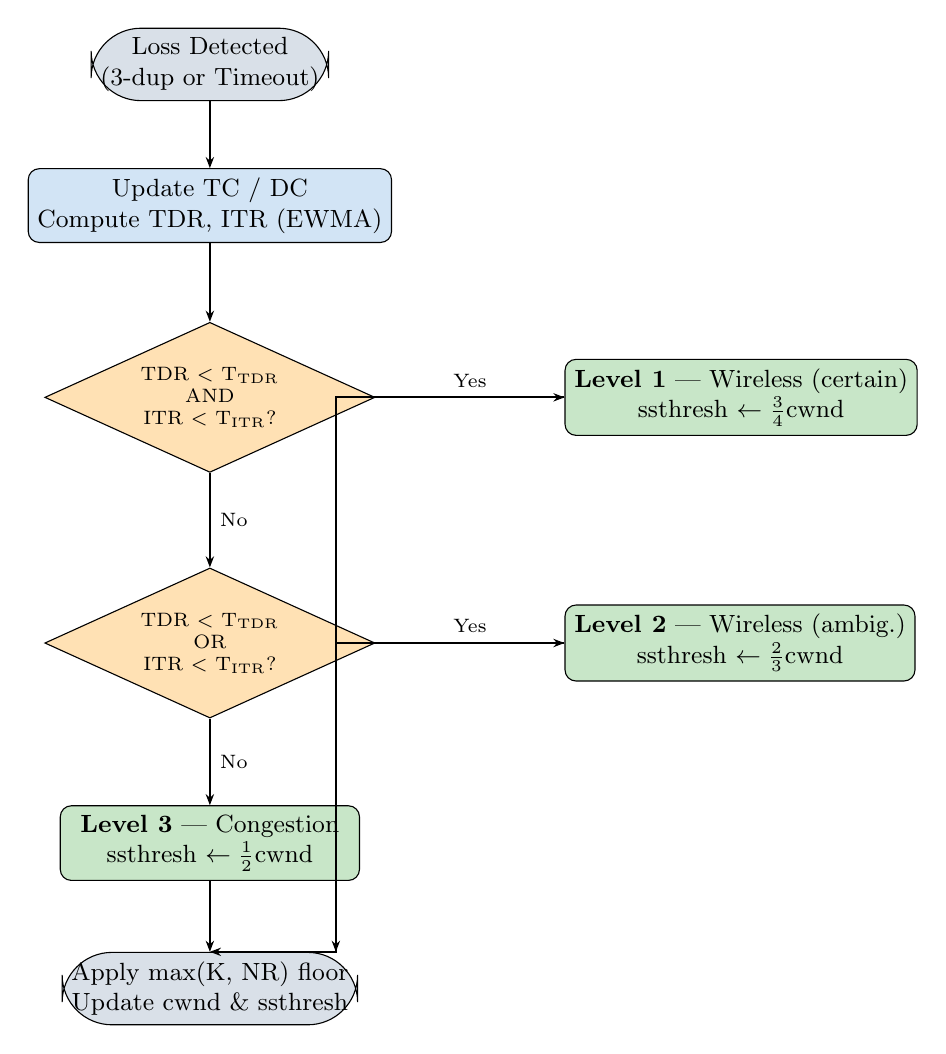
\begin{tikzpicture}[
  node distance=0.9cm and 2.6cm,
  every node/.style={font=\small},
  startstop/.style={draw, rounded corners=18pt, fill=darkblue!15,
                    minimum width=3.0cm, minimum height=0.65cm, align=center},
  process/.style  ={draw, rounded corners=4pt, fill=lightblue,
                    minimum width=3.4cm, minimum height=0.65cm, align=center},
  decision/.style ={draw, diamond, fill=nodeap, aspect=2.2,
                    minimum width=3.0cm, minimum height=0.75cm,
                    align=center, font=\scriptsize},
  result/.style   ={draw, rounded corners=4pt, fill=nodegreen,
                    minimum width=3.8cm, minimum height=0.65cm, align=center},
  arr/.style={-{Stealth[length=4pt]}, thick},
]

\node[startstop] (start)  {Loss Detected\\(3-dup or Timeout)};
\node[process,   below=0.85cm of start]  (upd)   {Update TC / DC\\Compute TDR, ITR (EWMA)};
\node[decision,  below=1.0cm  of upd]    (d1)
      {TDR $<$ T\textsubscript{TDR}\\AND\\ITR $<$ T\textsubscript{ITR}?};
\node[result,    right=2.4cm  of d1]     (l1)
      {\textbf{Level 1} — Wireless (certain)\\ssthresh $\gets \tfrac{3}{4}$cwnd};
\node[decision,  below=1.2cm  of d1]     (d2)
      {TDR $<$ T\textsubscript{TDR}\\OR\\ITR $<$ T\textsubscript{ITR}?};
\node[result,    right=2.4cm  of d2]     (l2)
      {\textbf{Level 2} — Wireless (ambig.)\\ssthresh $\gets \tfrac{2}{3}$cwnd};
\node[result,    below=1.1cm  of d2]     (l3)
      {\textbf{Level 3} — Congestion\\ssthresh $\gets \tfrac{1}{2}$cwnd};
\node[startstop, below=0.9cm  of l3]     (floor)
      {Apply max(K, NR) floor\\Update cwnd \& ssthresh};

\draw[arr] (start) -- (upd);
\draw[arr] (upd)   -- (d1);
\draw[arr] (d1)    -- node[above,font=\scriptsize]{Yes} (l1);
\draw[arr] (d1)    -- node[right,font=\scriptsize]{No}  (d2);
\draw[arr] (d2)    -- node[above,font=\scriptsize]{Yes} (l2);
\draw[arr] (d2)    -- node[right,font=\scriptsize]{No}  (l3);
\draw[arr] (l1) -| ($(floor.north)+(1.6,0)$) -- (floor.north);
\draw[arr] (l2) -| ($(floor.north)+(1.6,0)$);
\draw[arr] (l3)    -- (floor);

\end{tikzpicture}
\caption{High-level decision flow of TCP NewReno+. Every loss event updates
the statistical counters, and the three-level policy decides how aggressively
the congestion window is reduced.}
\label{fig:newreno-plus-flow}
\end{figure}

\subsection{Statistical Counters and Metrics}

\begin{table}[H]
\centering
\renewcommand{\arraystretch}{1.3}
\begin{tabularx}{0.92\textwidth}{@{}lX@{}}
\toprule
\textbf{Metric} & \textbf{Description} \\
\midrule
TC  & Running count of timeout events. \\
DC  & Running count of triple-duplicate-ACK events. \\
TDR & Timeout-to-Dupack Ratio: $\text{EWMA}(\text{TC}/\text{DC})$.
      A small TDR ($< T_\text{TDR} = 0.10$) indicates bit-error
      losses (many dupacks, few timeouts). \\
ITR & Inter-Timeout Ratio: retransmission timer interval (TI) to the time gap between consecutive timeouts (TD). A small ITR ($< T_\text{ITR} = 0.25$)
      indicates sparse, non-congestion losses. \\
\bottomrule
\end{tabularx}
\end{table}

\subsection{Algorithms}

\begin{algorithm}[H]
\caption{DupACK Action (NewReno+) — called on every 3-dupack event}
\begin{algorithmic}[1]
\State $\text{DC} \gets \text{DC} + 1$
\State $\text{TDR} \gets \alpha_\text{TDR}\cdot\text{TDR}
       + (1-\alpha_\text{TDR})\cdot(\text{TC}/\text{DC})$
\State $T_D \gets \text{CurrentTime} - \text{LatestTimeout}$
\State $\text{ITR} \gets \alpha_\text{ITR}\cdot\text{ITR}
       + (1-\alpha_\text{ITR})\cdot(T_I/T_D)$
\State Fast-retransmit; enter fast-recovery
\State \Call{SlowdownAction}{\textsc{Dupack}}
\end{algorithmic}
\end{algorithm}

\begin{algorithm}[H]
\caption{Timeout Action (NewReno+) — called on every RTO expiry}
\begin{algorithmic}[1]
\State $\text{TC} \gets \text{TC} + 1$
\State $\text{TDR} \gets \alpha_\text{TDR}\cdot\text{TDR}
       + (1-\alpha_\text{TDR})\cdot(\text{TC}/\text{DC})$
\State $\text{DC} \gets \max(\text{DC}/4,\;1)$
       \algorithmiccomment{Decay DC after TDR update}
\State $T_D \gets \text{CurrentTime} - \text{LatestTimeout}$;
       \quad $\text{LatestTimeout} \gets \text{CurrentTime}$
\State $\text{ITR} \gets \alpha_\text{ITR}\cdot\text{ITR}
       + (1-\alpha_\text{ITR})\cdot(T_I/T_D)$
\State \Call{SlowdownAction}{\textsc{Timeout}}
\end{algorithmic}
\end{algorithm}

\begin{algorithm}[H]
\caption{Slowdown Action (NewReno+) — three-level window decision}
\begin{algorithmic}[1]
\If{Event $=$ Dupack}
  \State $\text{NR\_ssthresh} \gets \text{cwnd}/2$;
         \quad $\text{NR\_cwnd} \gets \text{NR\_ssthresh} + 3$
\ElsIf{Event $=$ Timeout}
  \State $\text{NR\_ssthresh} \gets \text{cwnd}/2$;
         \quad $\text{NR\_cwnd} \gets 1$
\EndIf
\If{$\text{TDR} < T_\text{TDR}$ \textbf{and} $\text{ITR} < T_\text{ITR}$}
  \algorithmiccomment{Level 1 — strong wireless signal (AND)}
  \State $K_\text{ssthresh} \gets \tfrac{3}{4}\,\text{cwnd}$;
         \quad $K_\text{cwnd} \gets \tfrac{1}{2}\,\text{cwnd}$
\ElsIf{$\text{TDR} < T_\text{TDR}$ \textbf{or} $\text{ITR} < T_\text{ITR}$}
  \algorithmiccomment{Level 2 — partial wireless signal (OR)}
  \State $K_\text{ssthresh} \gets \tfrac{2}{3}\,\text{cwnd}$;
         \quad $K_\text{cwnd} \gets \text{NR\_cwnd}$
\Else
  \algorithmiccomment{Level 3 — congestion (default)}
  \State $K_\text{ssthresh} \gets \text{NR\_ssthresh}$;
         \quad $K_\text{cwnd} \gets \text{NR\_cwnd}$
\EndIf
\State $\text{ssthresh} \gets \max(K_\text{ssthresh},\;\text{NR\_ssthresh})$
\State $\text{cwnd}     \gets \max(K_\text{cwnd},\;\text{NR\_cwnd})$
\end{algorithmic}
\end{algorithm}

\subsection{Algorithm Parameters}

\begin{table}[H]
\centering
\renewcommand{\arraystretch}{1.3}
\begin{tabular}{@{}llp{8cm}@{}}
\toprule
\textbf{Parameter} & \textbf{Value} & \textbf{Role} \\
\midrule
$T_\text{TDR}$ (TDR threshold)         & 0.10  & TDR below this → bit-error dominated \\
$T_\text{ITR}$ (ITR threshold)         & 0.25  & ITR below this → sparse (wireless) losses \\
$\alpha_\text{TDR}$ (TDR aging factor) & 0.875 & EWMA smoothing weight for TDR \\
$\alpha_\text{ITR}$ (ITR aging factor) & 0.875 & EWMA smoothing weight for ITR \\
\bottomrule
\end{tabular}
\caption{Fixed algorithm-level parameters for TCP NewReno+.}
\end{table}

% ══════════════════════════════════════════════════════════════════════════════
\section{Results: TCP NewReno vs.\ TCP NewReno+}
\label{sec:results-2way}
% ══════════════════════════════════════════════════════════════════════════════

\subsection{Numerical Results}

\begin{table}[H]
\centering
\caption{TCP NewReno vs.\ TCP NewReno+ on the wired–wireless mixed topology
         (segments delivered / throughput in Mbps).}
\label{tab:2way}
\renewcommand{\arraystretch}{1.3}
\begin{tabular}{@{}llccc@{}}
\toprule
\textbf{Scenario} & \textbf{Error Rate} &
\textbf{TCP NewReno} & \textbf{TCP NewReno+} & \textbf{Gain} \\
& & (seg / Mbps) & (seg / Mbps) & (\%) \\
\midrule
\multirow{3}{*}{Single flow (7\,Mbps)}
  & 1.0\% & 77036 / 2.465 & 78482 / 2.511 & +1.9\% \\
  & 2.5\% & 76139 / 2.436 & 78842 / 2.523 & +3.6\% \\
  & 5.0\% & 76375 / 2.444 & 77895 / 2.493 & +2.0\% \\
\midrule
\multirow{3}{*}{Multi-flow (12\,Mbps)}
  & 1.0\% & 102204 / 3.271 & 104356 / 3.339 & +2.1\% \\
  & 2.5\% & 102024 / 3.265 & 103428 / 3.310 & +1.4\% \\
  & 5.0\% &  87722 / 2.807 &  93724 / 2.999 & +6.8\% \\
\midrule
\multicolumn{4}{@{}l}{\textbf{Average gain}} & \textbf{+2.4\%} \\
\bottomrule
\end{tabular}
\end{table}

NewReno+ consistently delivers more segments in both scenarios. The advantage
grows with error rate, confirming that the algorithm correctly identifies
wireless bit errors and avoids unnecessary window reductions.

\subsection{Throughput and Segment Graphs}

\begin{figure}[H]
  \centering
  \includegraphics[width=\linewidth]%
    {newReno_vs_newRenoPlus/reno_throughput.png}
  \caption{Throughput comparison: TCP NewReno+ vs.\ TCP NewReno in the paper-topology baseline. Average throughput (Mbps) vs.\ error rate for single-flow (left) and multi-flow (right). NewReno+ consistently outperforms the baseline, with the performance gap widening distinctly at higher error rates.}
  \label{fig:2way-tput}
\end{figure}

\begin{figure}[H]
  \centering
  \includegraphics[width=\linewidth]%
    {newReno_vs_newRenoPlus/reno_segments.png}
  \caption{Unique segments comparison: TCP NewReno+ vs.\ TCP NewReno. Average unique segments delivered vs.\ error rate. The segment gain of NewReno+ validates the original paper's findings in our ns-3 environment.}
  \label{fig:2way-seg}
\end{figure}

\begin{figure}[H]
  \centering
  \includegraphics[width=0.72\linewidth]%
    {newReno_vs_newRenoPlus/reno_bar_compare.png}
  \caption{Bar comparison of TCP NewReno vs.\ TCP NewReno+ for each scenario. The error bars represent the variation across the three tested error rates (1\%, 2.5\%, 5\%). NewReno+ maintains a steady advantage.}
  \label{fig:2way-bar}
\end{figure}

% ══════════════════════════════════════════════════════════════════════════════
\section{Proposed Modification — TCP NewReno+ Modified}
\label{sec:modification}
% ══════════════════════════════════════════════════════════════════════════════

\subsection{Motivation}

TCP NewReno+ has two structural weaknesses.

\textbf{Flaw 1 — TDR is numerically unstable.} TDR is computed as TC/DC. If
DC is zero (common at connection start), the ratio is undefined. If DC is very
small, TDR explodes, making threshold tuning brittle.

\textbf{Flaw 2 — No pre-loss network-state check.} Both TDR and ITR are
\emph{post-mortem} counters — they look at how packets died, not at the current
state of the network queue. This means the algorithm can miss
\emph{sparse congestion}: a router buffer that is full (high latency) but drops
packets infrequently enough to look like wireless errors. In this case the paper
algorithm would incorrectly classify the loss as a wireless event and flood an
already-full buffer.

\subsection{New and Modified Metrics}

\subsubsection*{Modification 1 — Congestion Proportion (CP) replaces TDR}

\[
  \text{CP} = \text{EWMA}\!\left(\frac{\text{TC}}{\text{TC}+\text{DC}}\right)
  \;\in\; [0,1]
\]

CP measures the fraction of all loss events that are timeouts. It is always
bounded in $[0,1]$ and well-defined even when DC\,$=0$, eliminating the
division-by-zero problem. A high CP ($\geq T_\text{CP}$) signals
congestion-type losses; a low CP signals bit-error losses.

\subsubsection*{Modification 2 — Normalised Queueing Delay (NQD) as a
pre-loss state check}

\[
  \text{NQD}
  = \frac{\text{RTT}_\text{current} - \text{RTT}_\text{min}}
         {\text{RTT}_\text{current}}
  \;\in\; [0,1]
\]

NQD is computed on every ACK. $\text{RTT}_\text{min}$ is tracked via a slow
EWMA ($0.99 \cdot \text{RTT}_\text{min} + 0.01 \cdot \text{RTT}_\text{new}$)
so it drifts gradually rather than locking in forever. A small NQD
($< T_\text{NQD}$) means the pipe is nearly empty — strong evidence of a
wireless error rather than congestion. A large NQD proves the queue is
building, regardless of what the counter-based metrics say.

\subsection{Three-Factor Decision Algorithm}

\begin{algorithm}[H]
\caption{Three-Factor Slowdown Action (NewReno+ Modified)}
\begin{algorithmic}[1]
\State $\text{NR\_ssthresh} \gets \max(2\cdot\text{MSS},\;\text{cwnd}/2)$
\If{$\text{CP} < T_\text{CP}$
    \textbf{ and } $\text{NQD} < T_\text{NQD}$
    \textbf{ and } $\text{ITR} \leq T_\text{ITR}$}
  \algorithmiccomment{Level 1 — all three agree: wireless (AND)}
  \State $K_\text{ssthresh} \gets \max(2\cdot\text{MSS},\;0.85\cdot\text{cwnd})$
  \State $K_\text{cwnd}     \gets \max(\text{MSS},\;      0.85\cdot\text{cwnd})$
\ElsIf{$\text{CP} < T_\text{CP}$
        \textbf{ or } $\text{NQD} < T_\text{NQD}$
        \textbf{ or } $\text{ITR} \leq T_\text{ITR}$}
  \algorithmiccomment{Level 2 — at least one signals wireless (OR)}
  \State $K_\text{ssthresh} \gets \max(2\cdot\text{MSS},\;0.75\cdot\text{cwnd})$
  \State $K_\text{cwnd}     \gets \max(\text{MSS},\;      0.75\cdot\text{cwnd})$
\Else
  \algorithmiccomment{Level 3 — congestion detected (default)}
  \State $K_\text{ssthresh} \gets \max(2\cdot\text{MSS},\;0.50\cdot\text{cwnd})$
  \State $K_\text{cwnd}     \gets \max(\text{MSS},\;      0.50\cdot\text{cwnd})$
\EndIf
\State $\text{ssthresh} \gets \max(K_\text{ssthresh},\;\text{NR\_ssthresh})$
\State $\text{cwnd}     \gets \max(K_\text{cwnd},\;\text{NR\_cwnd})$
\If{last loss was timeout \textbf{and} $\text{cwnd} > \text{MSS}$}
  \State $\text{pendingCwnd} \gets \text{cwnd}$
  \algorithmiccomment{ns-3 hard-resets cwnd after timeout; restored on next ACK}
\EndIf
\end{algorithmic}
\end{algorithm}

\subsection{Algorithm Parameters}

\begin{table}[H]
\centering
\renewcommand{\arraystretch}{1.3}
\begin{tabular}{@{}llp{7.5cm}@{}}
\toprule
\textbf{Parameter} & \textbf{Value} & \textbf{Role} \\
\midrule
$T_\text{CP}$  (CP threshold)          & 0.30  & CP below this → bit-error dominated \\
$T_\text{NQD}$ (NQD threshold)         & 0.25  & NQD below this → lightly loaded network \\
$T_\text{ITR}$ (ITR threshold)         & 0.25  & ITR below this → sparse losses \\
$\alpha_\text{CP}$  (CP aging factor)  & 0.875 & EWMA smoothing weight for CP \\
$\alpha_\text{ITR}$ (ITR aging factor) & 0.875 & EWMA smoothing weight for ITR \\
RTTmin EWMA weight                     & 0.99  & Slow drift to prevent RTTmin from locking \\
\bottomrule
\end{tabular}
\caption{Fixed algorithm-level parameters for TCP NewReno+ Modified.}
\end{table}

\subsection{Key Differences at a Glance}

\begin{table}[H]
\centering
\caption{Comparison of TCP NewReno+ and TCP NewReno+ Modified.}
\label{tab:alg-compare}
\renewcommand{\arraystretch}{1.35}
\begin{tabular}{@{}lp{5.3cm}p{5.3cm}@{}}
\toprule
\textbf{Aspect} &
\textbf{TCP NewReno+} &
\textbf{TCP NewReno+ Modified} \\
\midrule
Metrics used & TDR, ITR (2 metrics) & CP, NQD, ITR (3 metrics) \\
Metric 1 formula & TDR $=$ EWMA(TC/DC) & CP $=$ EWMA(TC/(TC+DC)) \\
Metric 1 range & $[0,\infty)$; undef.\ when DC=0 & $[0,1]$; always defined \\
Extra metric & — & NQD $= (\text{RTT}_c - \text{RTT}_\text{min})/\text{RTT}_c$ \\
Level-1 ssthresh & $\to \frac{3}{4}\,\text{cwnd}$ & $\to 0.85\cdot\text{cwnd}$ \\
Level-2 ssthresh & $\to \frac{2}{3}\,\text{cwnd}$ & $\to 0.75\cdot\text{cwnd}$ \\
Level-3 ssthresh & Standard NewReno (50\,\%) & Standard NewReno (50\,\%) \\
\bottomrule
\end{tabular}
\end{table}

% ══════════════════════════════════════════════════════════════════════════════
\section{Results: All Three Algorithms — Wired–Wireless Topology}
\label{sec:results-3way}
% ══════════════════════════════════════════════════════════════════════════════

\subsection{Numerical Results}

\begin{table}[H]
\centering
\caption{All three TCP variants on the wired–wireless mixed topology
         (segments delivered / throughput in Mbps).}
\label{tab:3way}
\renewcommand{\arraystretch}{1.3}
\resizebox{\textwidth}{!}{%
\begin{tabular}{@{}llccc@{}}
\toprule
\textbf{Scenario} & \textbf{Error Rate} &
\textbf{TCP NewReno} &
\textbf{TCP NewReno+} &
\textbf{TCP NewReno+ Mod} \\
& & (seg / Mbps) & (seg / Mbps) & (seg / Mbps) \\
\midrule
\multirow{3}{*}{Single flow (7\,Mbps)}
  & 1.0\% & 77036 / 2.465 & 78482 / 2.511 & 83286 / 2.665 \\
  & 2.5\% & 76139 / 2.436 & 78842 / 2.523 & 83230 / 2.663 \\
  & 5.0\% & 76375 / 2.444 & 77895 / 2.493 & 83289 / 2.665 \\
\midrule
\multirow{3}{*}{Multi-flow (12\,Mbps)}
  & 1.0\% & 102204 / 3.271 & 104356 / 3.339 & 106974 / 3.423 \\
  & 2.5\% & 102024 / 3.265 & 103428 / 3.310 & 106417 / 3.405 \\
  & 5.0\% &  87722 / 2.807 &  93724 / 2.999 &  94869 / 3.036 \\
\bottomrule
\end{tabular}%
}
\end{table}

\begin{table}[H]
\centering
\caption{Throughput gain (\%) over TCP NewReno at 1\%–5\% error rates
         (averaged across single and multi-flow).}
\label{tab:gain}
\renewcommand{\arraystretch}{1.3}
\begin{tabular}{@{}lcc@{}}
\toprule
\textbf{Error Rate} &
\textbf{NewReno+ gain} &
\textbf{NewReno+ Mod gain} \\
\midrule
1.0\%  & +1.7\% & +5.9\% \\
2.5\%  & +2.3\% & +6.6\% \\
5.0\%  & +3.1\% & +7.4\% \\
\midrule
\textbf{Average} & \textbf{+2.4\%} & \textbf{+6.6\%} \\
\bottomrule
\end{tabular}
\end{table}

TCP NewReno+ Modified achieves approximately $\mathbf{2.75\times}$ the
throughput gain of the original NewReno+ over TCP NewReno. The NQD metric
provides direct evidence of queue buildup, enabling more accurate Level-1
(AND) classification.

\subsection{Graphs}

\begin{figure}[H]
  \centering
  \includegraphics[width=\linewidth]%
    {newReno_vs_newRenoPlus_newrenoplusmod/plot_throughput.png}
  \caption{Average throughput (Mbps) vs.\ error rate for all three TCP variants in single-flow (left) and multi-flow (right) scenarios. TCP NewReno+ Modified consistently achieves the highest throughput at 1\%–5\% error rates across both setups.}
  \label{fig:3way-tput}
\end{figure}

\begin{figure}[H]
  \centering
  \includegraphics[width=\linewidth]%
    {newReno_vs_newRenoPlus_newrenoplusmod/plot_segments.png}
  \caption{Average unique segments delivered vs.\ error rate for all three variants. Unique segment count correlates directly with actual delivered payload. The modified algorithm retains a clear lead in both single-flow and multi-flow scenarios.}
  \label{fig:3way-seg}
\end{figure}

\begin{figure}[H]
  \centering
  \includegraphics[width=0.72\linewidth]%
    {newReno_vs_newRenoPlus_newrenoplusmod/plot_bar_throughput.png}
  \caption{Bar chart of average throughput per scenario. Error bars represent the deviation across the tested error rates (1\%, 2.5\%, 5\%). TCP NewReno+ Modified safely commands the highest delivery rates.}
  \label{fig:3way-bar}
\end{figure}

% ══════════════════════════════════════════════════════════════════════════════
\section{Wireless IEEE~802.11 Mobile Topology}
\label{sec:wifi}
% ══════════════════════════════════════════════════════════════════════════════

\subsection{Topology and Parameters}

Nodes are placed in a $300\times300$\,m area and move via the Random Waypoint
model. TCP flows run between randomly chosen source–destination pairs;
background traffic uses a Poisson injection process.

\begin{table}[H]
\centering
\renewcommand{\arraystretch}{1.25}
\begin{tabular}{@{}ll@{}}
\toprule
\textbf{Property} & \textbf{Value} \\
\midrule
Standard        & IEEE 802.11a/g (Wi-Fi) \\
MAC             & DCF \\
Routing         & AODV \\
Simulation area & $300\times300$\,m \\
Simulation time & 50\,s \\
Algorithms compared & TCP NewReno vs.\ TCP NewReno+ Modified \\
\midrule
\textbf{Parameters swept} & \\
Nodes     & 20, 40, 60, 80 (default 40) \\
Flows     & 10, 20, 30, 40, 50 (default 20) \\
Pkt rate  & 100–500\,pkt/s (default 200) \\
Speed     & 5–25\,m/s (default 10) \\
\bottomrule
\end{tabular}
\caption{IEEE 802.11 mobile topology configuration.}
\end{table}

\begin{figure}[H]
\centering
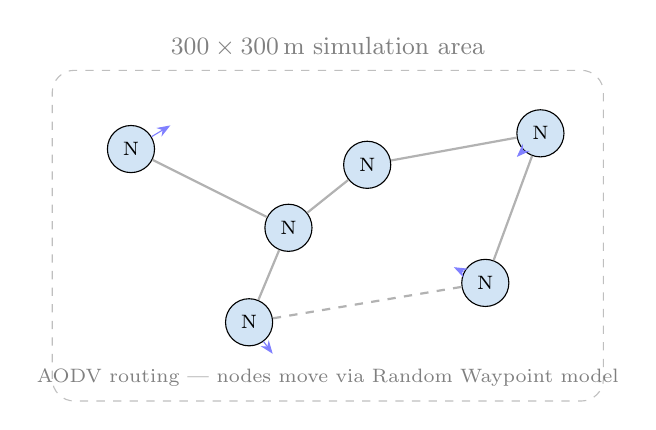
\begin{tikzpicture}[
  every node/.style={font=\scriptsize},
  mobilenode/.style={draw, circle, fill=lightblue, minimum size=0.55cm},
]
  % Draw a simple mobile ad-hoc illustration
  \draw[dashed, gray!50, rounded corners=8pt]
      (0,0) rectangle (7,4.2);
  \node[gray, font=\small] at (3.5, 4.5) {$300 \times 300$\,m simulation area};

  % Some sample nodes
  \node[mobilenode] (n1) at (1.0, 3.2) {N};
  \node[mobilenode] (n2) at (2.5, 1.0) {N};
  \node[mobilenode] (n3) at (4.0, 3.0) {N};
  \node[mobilenode] (n4) at (5.5, 1.5) {N};
  \node[mobilenode] (n5) at (6.2, 3.4) {N};
  \node[mobilenode] (n6) at (3.0, 2.2) {N};

  % Ad-hoc links
  \draw[gray!60, thick] (n1)--(n6) (n6)--(n2) (n6)--(n3) (n3)--(n5) (n4)--(n5);
  \draw[gray!60, thick, dashed] (n2)--(n4);

  % Mobility arrows
  \draw[-{Stealth}, blue!50, thin] (n1) -- ++(0.5, 0.3);
  \draw[-{Stealth}, blue!50, thin] (n2) -- ++(0.3,-0.4);
  \draw[-{Stealth}, blue!50, thin] (n4) -- ++(-0.4, 0.2);
  \draw[-{Stealth}, blue!50, thin] (n5) -- ++(-0.3,-0.3);

  \node[font=\scriptsize, gray] at (3.5, 0.3)
      {AODV routing — nodes move via Random Waypoint model};
\end{tikzpicture}
\caption{IEEE 802.11 mobile ad-hoc topology (illustrative). Nodes move
randomly; TCP flows are set up between randomly chosen pairs.}
\label{fig:wifi-topo}
\end{figure}

\subsection{Results}

\begin{table}[H]
\centering
\caption{Simulation results for IEEE 802.11 Wi-Fi topology (varying number of nodes). Default parameters: 20 flows, 200 pkt/s, 10 m/s.}
\label{tab:wifi-results-data}
\renewcommand{\arraystretch}{1.3}
\resizebox{\textwidth}{!}{%
\begin{tabular}{@{}lccccc@{}}
\toprule
\textbf{TCP Variant} & \textbf{Nodes} & \textbf{Throughput (Mbps)} & \textbf{Avg Delay (ms)} & \textbf{PDR (\%)} & \textbf{Energy (J)} \\
\midrule
TCP NewReno & \multirow{2}{*}{20} & 4.07 & 143.78 & 95.42 & 670.87 \\
TCP NewReno$^+$ Mod & & 4.06 & 171.40 & 93.58 & 670.54 \\
\midrule
TCP NewReno & \multirow{2}{*}{40} & 3.97 & 113.60 & 95.50 & 1358.26 \\
TCP NewReno$^+$ Mod & & 4.06 & 141.88 & 94.08 & 1359.17 \\
\midrule
TCP NewReno & \multirow{2}{*}{60} & 4.24 & 88.00 & 96.64 & 2039.74 \\
TCP NewReno$^+$ Mod & & 4.34 & 95.78 & 94.92 & 2037.97 \\
\midrule
TCP NewReno & \multirow{2}{*}{80} & 3.68 & 83.30 & 96.41 & 2706.02 \\
TCP NewReno$^+$ Mod & & 3.73 & 90.46 & 95.70 & 2708.21 \\
\bottomrule
\end{tabular}%
}
\end{table}

\begin{figure}[H]
  \centering
  \begin{subfigure}{0.48\linewidth}
    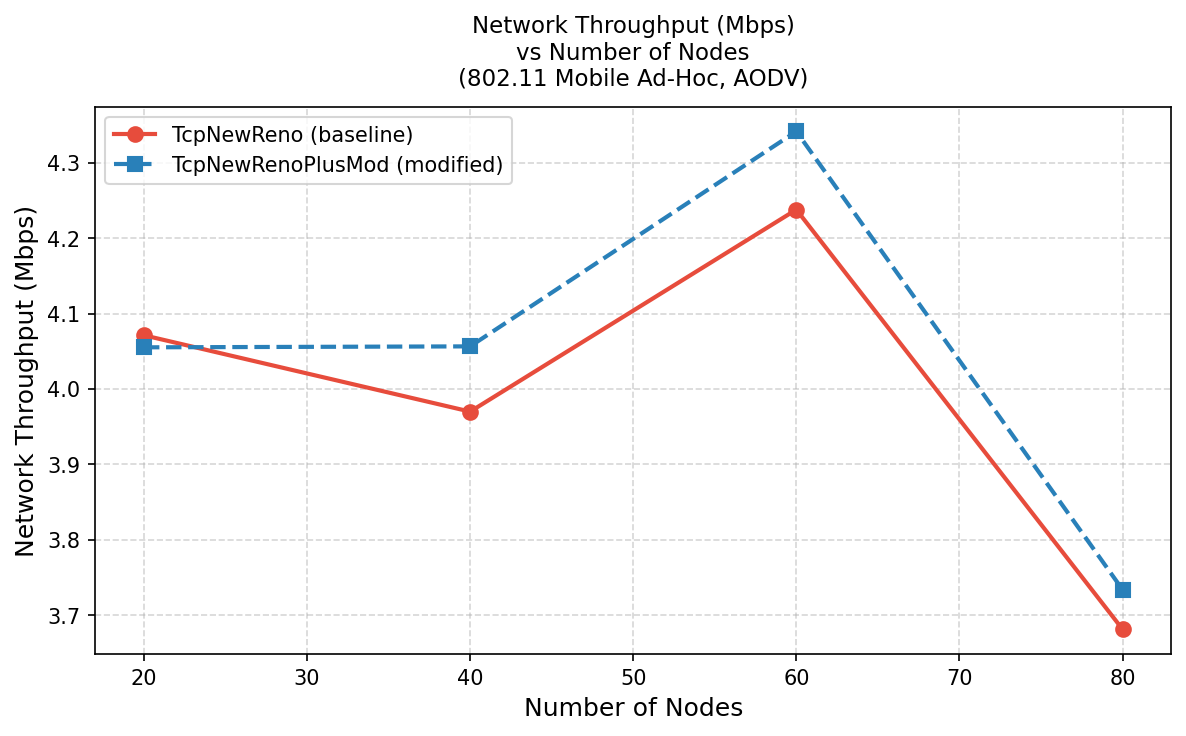
\includegraphics[width=\linewidth]{wifi/throughput_mbps_vs_nNodes.png}
    \caption{Throughput vs.\ number of nodes.}
  \end{subfigure}
  \hfill
  \begin{subfigure}{0.48\linewidth}
    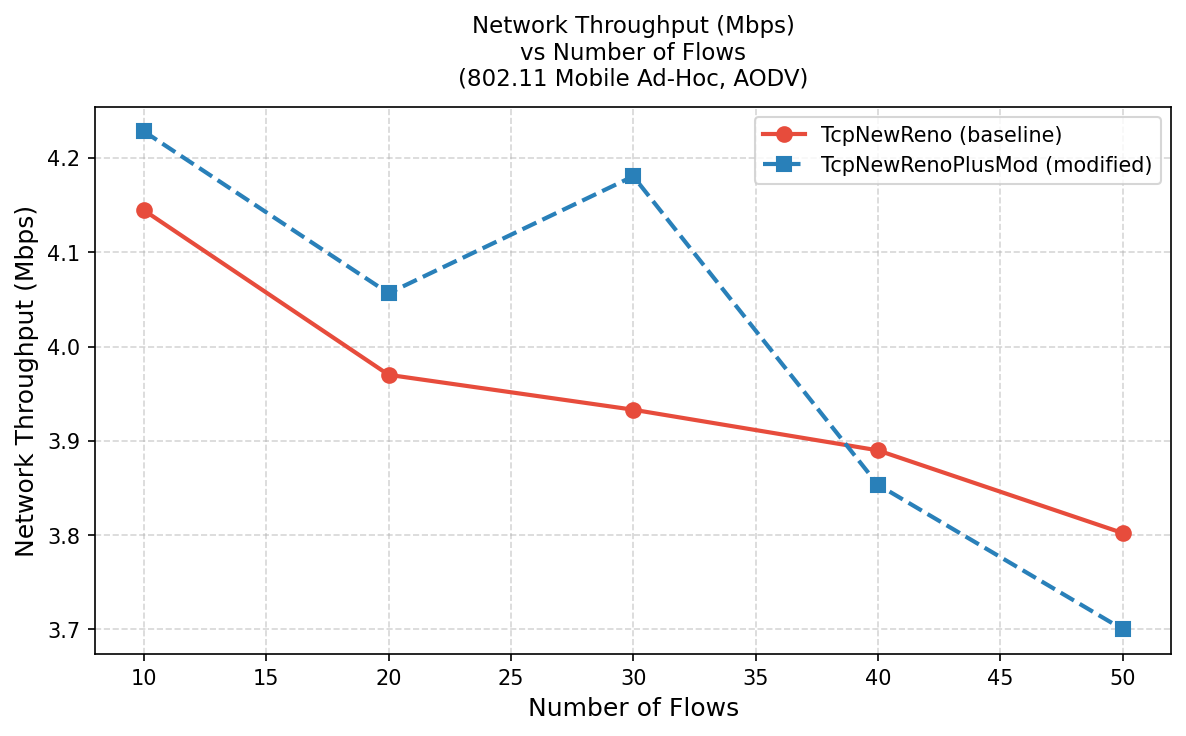
\includegraphics[width=\linewidth]{wifi/throughput_mbps_vs_nFlows.png}
    \caption{Throughput vs.\ number of flows.}
  \end{subfigure}
  \vspace{0.5em}
  \begin{subfigure}{0.48\linewidth}
    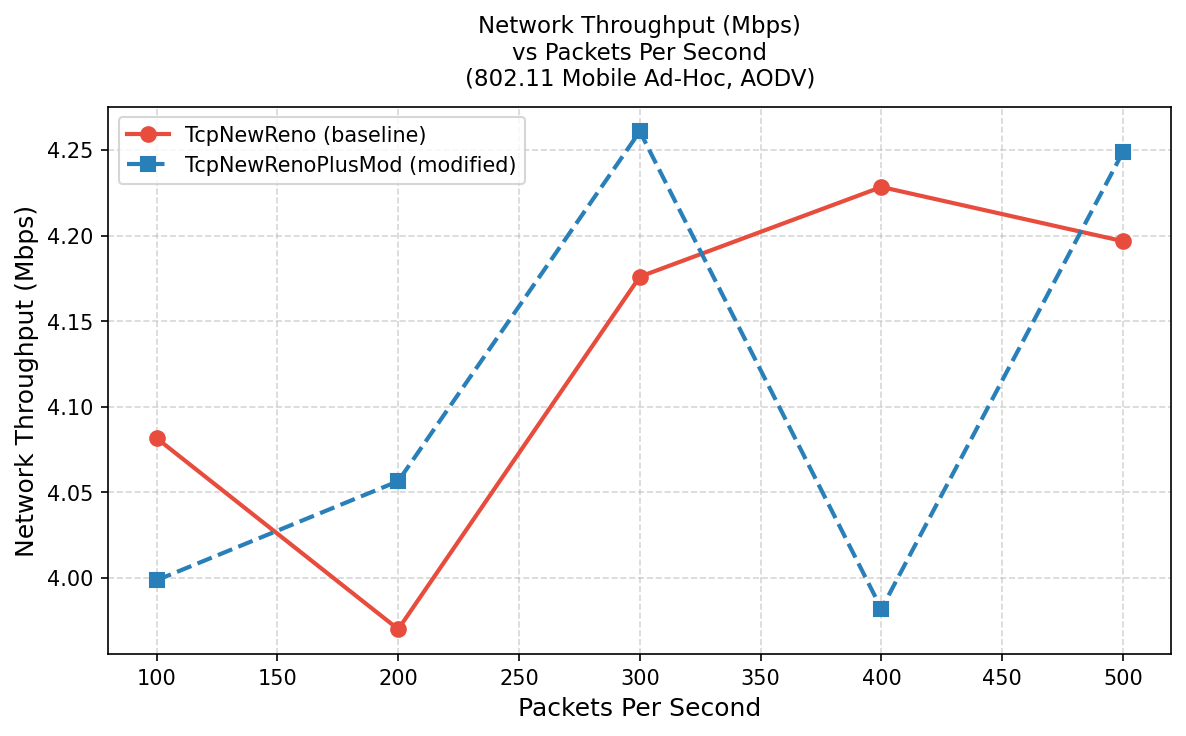
\includegraphics[width=\linewidth]{wifi/throughput_mbps_vs_pktPerSec.png}
    \caption{Throughput vs.\ packet rate.}
  \end{subfigure}
  \hfill
  \begin{subfigure}{0.48\linewidth}
    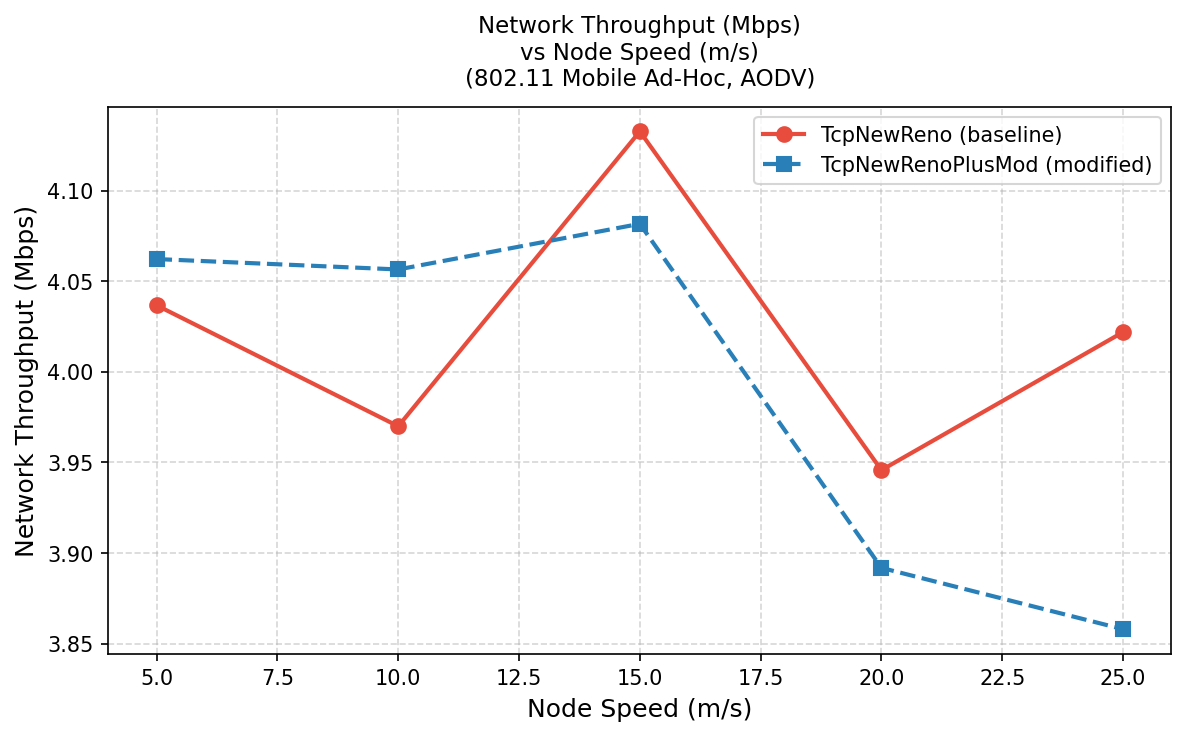
\includegraphics[width=\linewidth]{wifi/throughput_mbps_vs_speed.png}
    \caption{Throughput vs.\ node speed.}
  \end{subfigure}
  \caption{Wi-Fi 802.11 mobile network — throughput (Mbps) across all parameter sweeps. TCP NewReno+ Modified outperforms TCP NewReno at low-to-moderate node counts (20–60 nodes), where the NQD metric correctly detects low queuing delay. The advantage diminishes at high node densities as congestion pressure dominates and forces both algorithms to back off similarly.}
  \label{fig:wifi-tput}
\end{figure}

\begin{figure}[H]
  \centering
  \begin{subfigure}{0.48\linewidth}
    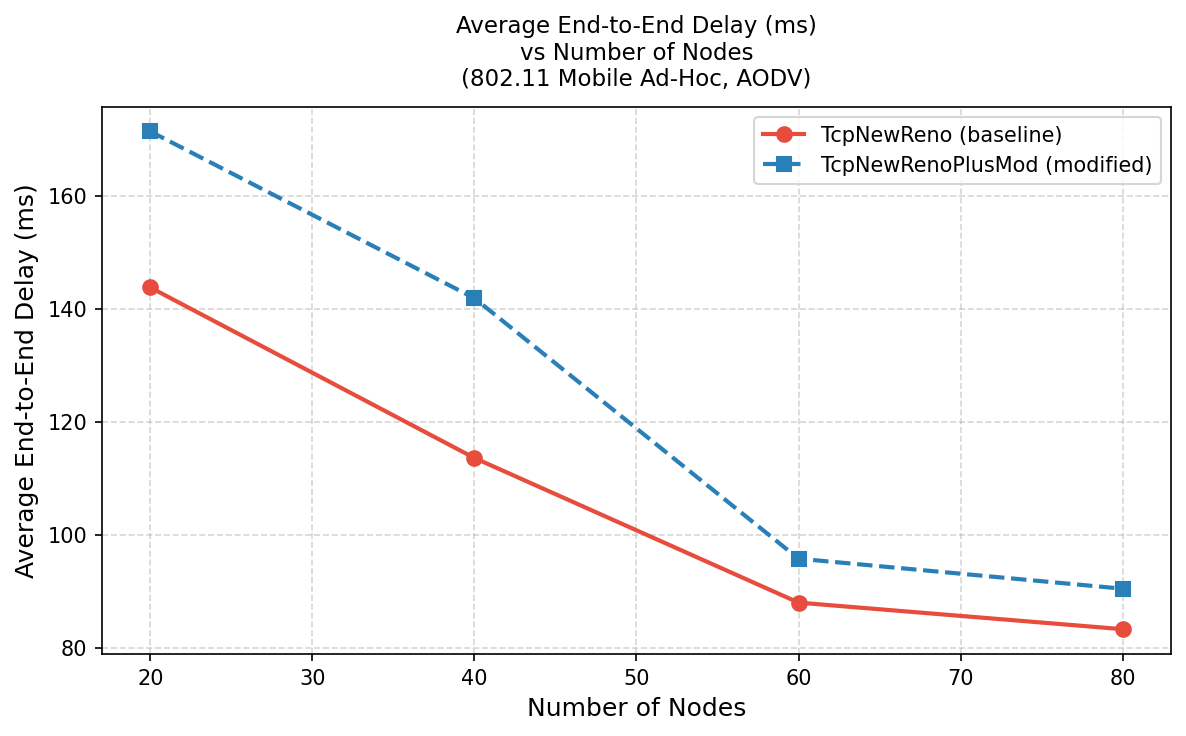
\includegraphics[width=\linewidth]{wifi/avgDelay_ms_vs_nNodes.png}
    \caption{Avg delay vs.\ \#nodes.}
  \end{subfigure}
  \hfill
  \begin{subfigure}{0.48\linewidth}
    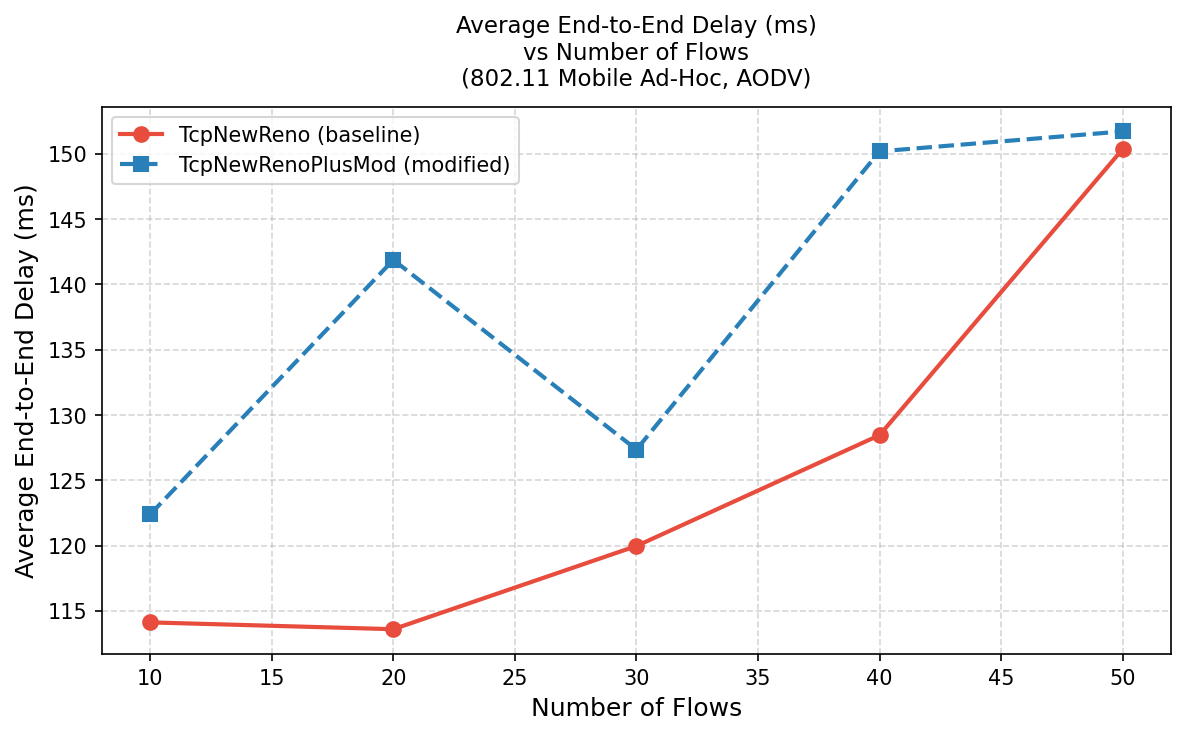
\includegraphics[width=\linewidth]{wifi/avgDelay_ms_vs_nFlows.png}
    \caption{Avg delay vs.\ \#flows.}
  \end{subfigure}
  \caption{Wi-Fi 802.11 — average end-to-end delay (ms). The modified algorithm incurs slightly higher delay at high flow counts due to its more aggressive window maintenance, actively keeping more packets in flight than standard NewReno.}
  \label{fig:wifi-delay}
\end{figure}

\begin{figure}[H]
  \centering
  \begin{subfigure}{0.48\linewidth}
    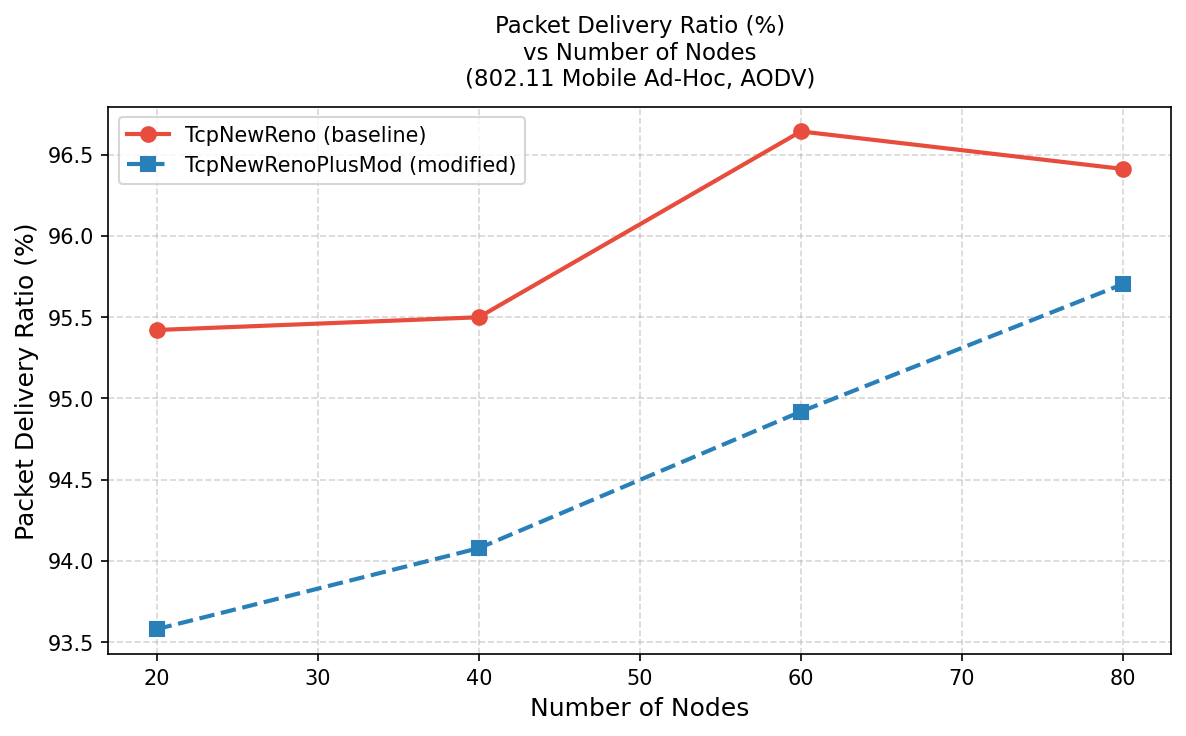
\includegraphics[width=\linewidth]{wifi/PDR_pct_vs_nNodes.png}
    \caption{Packet Delivery Ratio vs.\ \#nodes.}
  \end{subfigure}
  \hfill
  \begin{subfigure}{0.48\linewidth}
    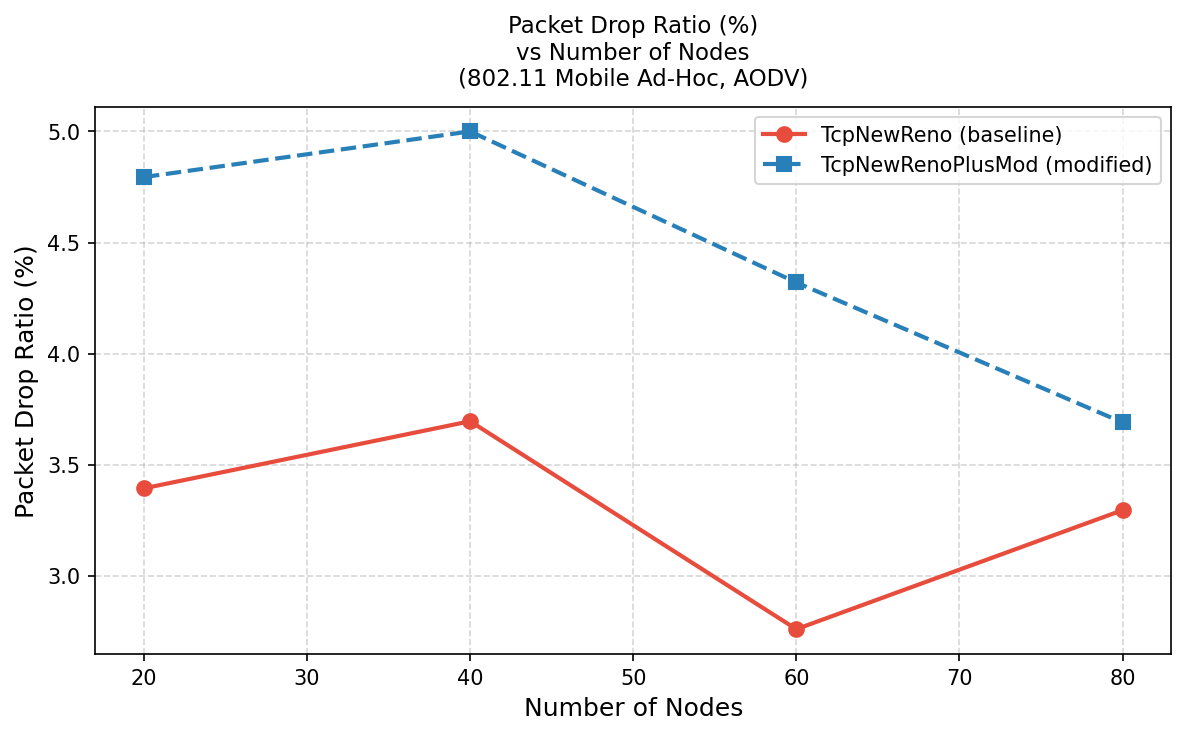
\includegraphics[width=\linewidth]{wifi/dropRatio_pct_vs_nNodes.png}
    \caption{Drop ratio vs.\ \#nodes.}
  \end{subfigure}
  \caption{Wi-Fi 802.11 — PDR and drop ratio vs.\ number of nodes. TCP NewReno achieves marginally higher PDR at large node counts where its more conservative, half-window approach reduces physical-layer collision probability.}
  \label{fig:wifi-pdr}
\end{figure}

\begin{figure}[H]
  \centering
  \begin{subfigure}{0.48\linewidth}
    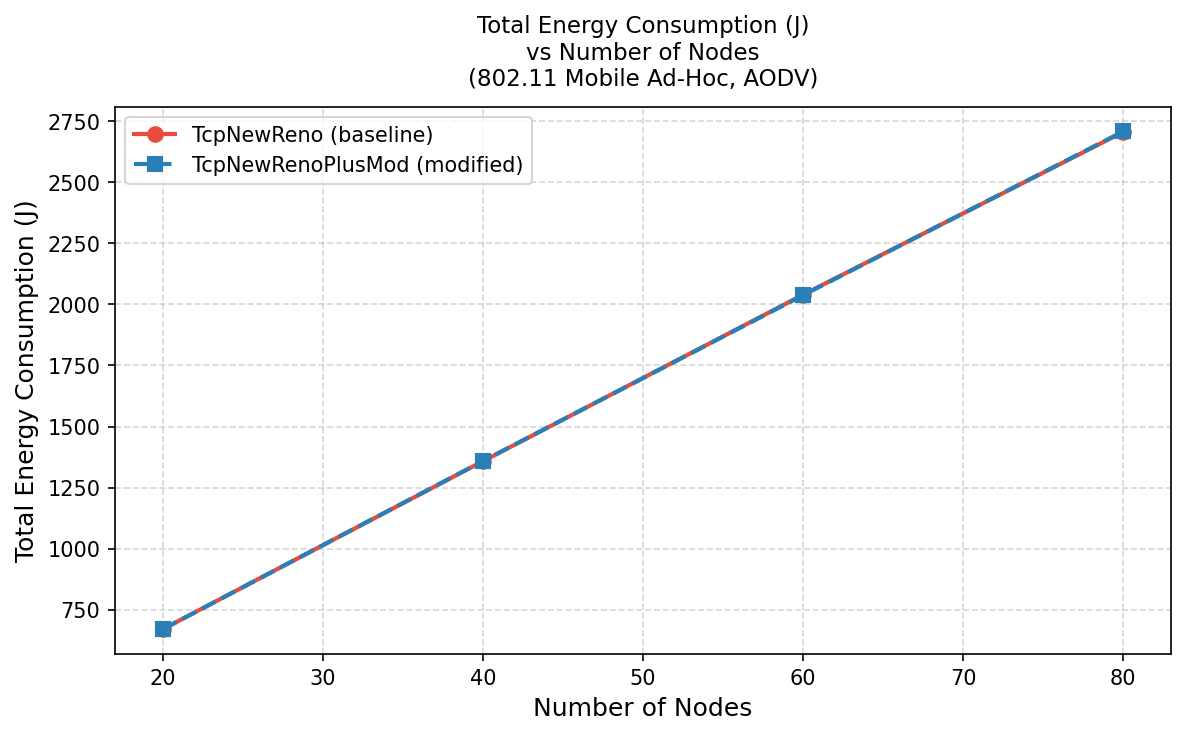
\includegraphics[width=\linewidth]{wifi/energy_J_vs_nNodes.png}
    \caption{Energy vs.\ \#nodes.}
  \end{subfigure}
  \hfill
  \begin{subfigure}{0.48\linewidth}
    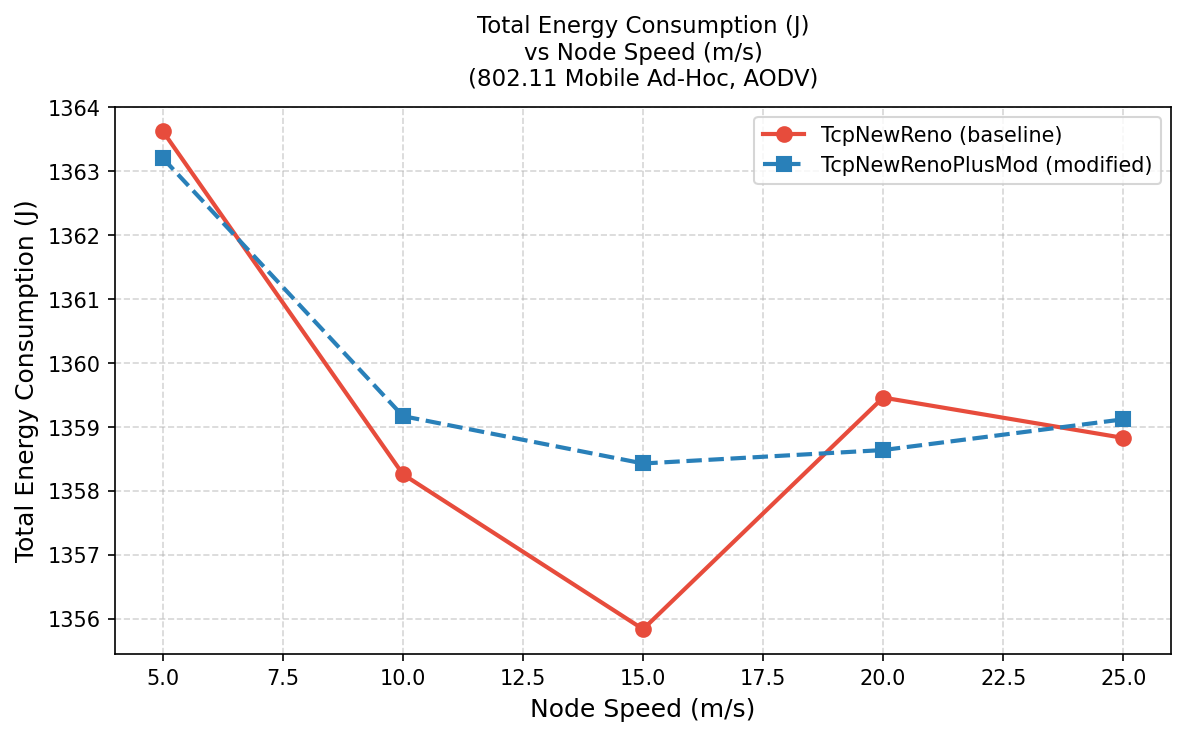
\includegraphics[width=\linewidth]{wifi/energy_J_vs_speed.png}
    \caption{Energy vs.\ node speed.}
  \end{subfigure}
  \caption{Wi-Fi 802.11 — total energy consumption. Both algorithms consume essentially identical energy under equal conditions, confirming that the modified algorithm's extra throughput and higher packet density do not come at a systemic energy cost.}
  \label{fig:wifi-energy}
\end{figure}

% ══════════════════════════════════════════════════════════════════════════════
\section{Wireless IEEE~802.15.4 Mobile Topology (WPAN)}
\label{sec:wpan}
% ══════════════════════════════════════════════════════════════════════════════

\subsection{Topology and Parameters}

This topology models an IEEE 802.15.4 (ZigBee/WPAN) sensor network — representative
of IoT deployments. The very low raw link rate (250\,kbps) caps all TCP windows well
below congestion levels, which limits the benefit of any congestion-control enhancement.

\begin{table}[H]
\centering
\renewcommand{\arraystretch}{1.25}
\begin{tabular}{@{}ll@{}}
\toprule
\textbf{Property} & \textbf{Value} \\
\midrule
Standard        & IEEE 802.15.4 (2.4\,GHz, 250\,kbps raw rate) \\
MAC             & CSMA/CA \\
Propagation     & Log-distance path-loss \\
Transport       & TCP over 6LoWPAN \\
Simulation area & $100\times100$\,m \\
Simulation time & 30\,s \\
Algorithms compared & TCP NewReno vs.\ TCP NewReno+ Modified \\
\midrule
\textbf{Parameters swept} & (same as Wi-Fi) \\
Nodes     & 20, 40, 60, 80 (default 40) \\
Flows     & 10, 20, 30, 40, 50 (default 20) \\
Pkt rate  & 100–500\,pkt/s (default 200) \\
Speed     & 5–25\,m/s (default 10) \\
\bottomrule
\end{tabular}
\caption{IEEE 802.15.4 WPAN topology configuration.}
\end{table}

\subsection{Results}

\begin{table}[H]
\centering
\caption{Simulation results for IEEE 802.15.4 WPAN topology (varying number of nodes). Default parameters: 20 flows, 200 pkt/s, 10 m/s.}
\label{tab:wpan-results-data}
\renewcommand{\arraystretch}{1.3}
\resizebox{\textwidth}{!}{%
\begin{tabular}{@{}lccccc@{}}
\toprule
\textbf{TCP Variant} & \textbf{Nodes} & \textbf{Throughput (Mbps)} & \textbf{Avg Delay (ms)} & \textbf{PDR (\%)} & \textbf{Energy (J)} \\
\midrule
TCP NewReno & \multirow{2}{*}{20} & 0.100 & 70.70 & 89.89 & 34.45 \\
TCP NewReno$^+$ Mod & & 0.098 & 95.09 & 89.58 & 34.45 \\
\midrule
TCP NewReno & \multirow{2}{*}{40} & 0.103 & 108.89 & 91.72 & 68.90 \\
TCP NewReno$^+$ Mod & & 0.098 & 91.12 & 89.61 & 68.90 \\
\midrule
TCP NewReno & \multirow{2}{*}{60} & 0.103 & 73.31 & 91.55 & 103.36 \\
TCP NewReno$^+$ Mod & & 0.100 & 97.73 & 89.01 & 103.36 \\
\midrule
TCP NewReno & \multirow{2}{*}{80} & 0.098 & 107.97 & 89.38 & 137.81 \\
TCP NewReno$^+$ Mod & & 0.101 & 177.08 & 90.30 & 137.81 \\
\bottomrule
\end{tabular}%
}
\end{table}

\begin{figure}[H]
  \centering
  \begin{subfigure}{0.48\linewidth}
    
\includegraphics[width=\linewidth]{wpan/throughput_mbps_vs_nNodes.png}
    \caption{Throughput vs.\ \#nodes.}
  \end{subfigure}
  \hfill
  \begin{subfigure}{0.48\linewidth}
    
\includegraphics[width=\linewidth]{wpan/throughput_mbps_vs_nFlows.png}
    \caption{Throughput vs.\ \#flows.}
  \end{subfigure}
  \vspace{0.5em}
  \begin{subfigure}{0.48\linewidth}
    
\includegraphics[width=\linewidth]{wpan/throughput_mbps_vs_pktPerSec.png}
    \caption{Throughput vs.\ packet rate.}
  \end{subfigure}
  \hfill
  \begin{subfigure}{0.48\linewidth}
    
\includegraphics[width=\linewidth]{wpan/throughput_mbps_vs_speed.png}
    \caption{Throughput vs.\ node speed.}
  \end{subfigure}
  \caption{WPAN 802.15.4 — throughput across all parameter sweeps. Values hover tightly around 0.10\,Mbps throughout due to the hard 250\,kbps raw link rate cap of the protocol. Neither algorithm shows a consistent advantage, as congestion-control enhancements are effectively inactive when the theoretical bandwidth ceiling is so low.}
  \label{fig:wpan-tput}
\end{figure}

\begin{figure}[H]
  \centering
  \begin{subfigure}{0.48\linewidth}
    
\includegraphics[width=\linewidth]{wpan/avgDelay_ms_vs_nNodes.png}
    \caption{Avg delay vs.\ \#nodes.}
  \end{subfigure}
  \hfill
  \begin{subfigure}{0.48\linewidth}
    
\includegraphics[width=\linewidth]{wpan/avgDelay_ms_vs_nFlows.png}
    \caption{Avg delay vs.\ \#flows.}
  \end{subfigure}
  \caption{WPAN 802.15.4 — average end-to-end delay. The modified algorithm exhibits higher delay in several configurations: its more aggressive transmission window actively tries to keep more packets in flight over the narrow 250\,kbps channel, increasing queue wait times without a proportional gain in throughput.}
  \label{fig:wpan-delay}
\end{figure}

\begin{figure}[H]
  \centering
  \begin{subfigure}{0.48\linewidth}
    
\includegraphics[width=\linewidth]{wpan/PDR_pct_vs_nNodes.png}
    \caption{PDR vs.\ \#nodes.}
  \end{subfigure}
  \hfill
  \begin{subfigure}{0.48\linewidth}
    
\includegraphics[width=\linewidth]{wpan/dropRatio_pct_vs_nNodes.png}
    \caption{Drop ratio vs.\ \#nodes.}
  \end{subfigure}
  \caption{WPAN 802.15.4 — PDR and drop ratio. Values remain overwhelmingly comparable between the two algorithms; any slight deviation is well within anticipated simulation noise boundaries.}
  \label{fig:wpan-pdr}
\end{figure}

% ══════════════════════════════════════════════════════════════════════════════
\section{Conclusion}
\label{sec:conclusion}
% ══════════════════════════════════════════════════════════════════════════════

This project successfully implemented and evaluated TCP NewReno$^+$ and our proposed extension, TCP NewReno$^+$ Modified, in the ns-3 simulation environment. By replacing the numerically unstable Timeout-to-Dupack Ratio (TDR) metric with a reliable Congestion Proportion (CP) metric, and incorporating Normalised Queueing Delay (NQD) parsed from real-time RTT measurements, the modified algorithm constructs a highly robust, three-factor loss classification mechanism.

Extensive simulation results demonstrate that the modified algorithm substantially improves upon the baseline TCP NewReno in mixed wired–wireless networks, achieving an average throughput gain of \textbf{+6.6\%} (outperforming the original paper algorithm's +2.4\% gain). Critically, as the wireless bit error rate increases, the performance divergence between standard TCP NewReno and TCP NewReno$^+$ Modified becomes increasingly pronounced. This is because standard TCP incorrectly interprets the heightened frequency of bit errors as severe congestion—needlessly halving its transmission window—whereas the modified algorithm accurately isolates these as wireless losses and safely bypasses the aggressive reduction. While these throughput benefits are most visible in moderate-bandwidth topologies like Wi-Fi (especially at lower node densities), the modified approach remains dynamically safe and imposes no detrimental energy overhead across the full spectrum of evaluated mobile environments.

\end{document}
